\subsubsection{Minuta de reunião (09-Setembro-2015)}

\begin{tabbing}
  Local \= xxx \kill
  Local \> : LEAD \\
  Data  \> : 09 de Setembro de 2015 \\
  Hora  \> : 13:00
\end{tabbing}

%---------------------------------------------------------------------
\participantes{
  \alana
  \gabriel,
  \julia,
  \estevão,
  \elael,
  \renan,
  \ramon.

}

\textbf{Aprovação da minuta}

\textbf{Update semanal do Projeto EMMA}
   							
\textbf{\alana.} 
	\begin{itemize}
		\item \textbf{Tarefas concluídas:}
			\begin{itemize}    
				\item Ofício Viagem Jirau: passagens, diárias e locação de carros.
				\item Cronograma de viagem.
				\item Justificativa Ramon.
			\end{itemize}
		
		\item \textbf{Novas tarefas:}
			\begin{itemize} 
				\item Coordenar com Gizele (ESBR) detalhes da viagem.
			\end{itemize}
	\end{itemize}   		
						
\textbf{\gabriel.} 
	\begin{itemize}
			\item Trabalhou no alinhamento da nuvem de pontos.
			\item Fez estudo sobre alinhamento de pás e braço mecânico para auxiliar o
			trabalho de dinâmica do Renan.
			\end{itemize}
		
		\item \textbf{Novas tarefas:}
			\begin{itemize} 
				\item Continuar trabalhando com alinhamento de point cloud. Cruzamento de
				modelos e informações diferentes que possam satisfazer provar a viabilidade
				de sensores na atividade de calibração.
			\end{itemize}

					
			
   \textbf{\estevão.} 
	\begin{itemize}
		\item \textbf{Tarefas concluídas:}
			\begin{itemize}  
			  \item Apresentação de possíveis soluções modulares para bases robóticas em
			  ambientes de difícil acesso.
			\end{itemize}
		
		\item \textbf{Novas tarefas:}
			\begin{itemize} 
				\item Continuar estudo de bases e sua logística em ambientes confinados.
			\end{itemize}
	\end{itemize}

	  \textbf{\renan.} 
	\begin{itemize}
		\item \textbf{Tarefas concluídas:}
			\begin{itemize}    
				\item Continuou apresentação do estudo de dinâmica.
			\end{itemize}
		
		\item \textbf{Novas tarefas:}
			\begin{itemize} 
			    \item Adicionar um estudo de discretizaçào da pá.
			\end{itemize}
	\end{itemize}	
	
	
	  \textbf{\elael.} 
	\begin{itemize}
		\item \textbf{Tarefas concluídas:}
			\begin{itemize}    
				\item Reuniu elementos apra apresentação em Jirau antes de sair de férias.
			\end{itemize}
		
			
   \textbf{\julia.} 
	\begin{itemize}
		\item \textbf{Tarefas concluídas:}
			\begin{itemize}    
				\item Apresentação processo de trabalho para EMMA Fase 2: Design.
				\item Coordenar material para apresentações em Jirau.
			\end{itemize}
		
		\item \textbf{Novas tarefas:}
			\begin{itemize} 

			    \item Apresentar Fase 3: Desenvolvimento.
			\end{itemize}
	\end{itemize}		



\textbf{Agenda para a próxima reunião:}
  \begin{itemize}
    \item Resultado de pesquisas individuais.
    \item Novas tarefas \& recomendações.
  \end{itemize}


\vspace{5mm}%
\parbox[t]{70mm}{
  Aprovado por: \\[5mm]
  \centering
  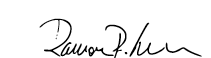
\includegraphics[width=65mm]{figs/logo/assinatura-ramon.png} \\[-4mm]
  \rule[2mm]{70mm}{0.1mm} \\
  \ramon \\[1mm]
  Coordenador do Projeto \\
}

%---------------------------------------------------------------------
\fim